
% this file is called up by thesis.tex
% content in this file will be fed into the main document

%: ----------------------- introduction file header -----------------------
\chapter{Cross-lingual Document Similarity}\label{ch:multilinguality}

\graphicspath{{multilinguality/figures/}}

% -------------------------------------------------------------
% -- Multilinguality
% -------------------------------------------------------------
% - Mimno et al., 2009. Polylingual topic models.
% - Jagarlamudi & Daume III, 2010. Extracting multilingual topics from unaligned comparable corpora.
% - Boyd-Graber & Resnik, 2010. Holistic sentiment analysis across languages: Multilingual supervised latent Dirichlet allocation.
% - Shi et al., 2016. Detecting common discussion topics across culture from news reader comments. 
% - Hao & Paul, 2018. Learning Multilingual Topics from Incomparable Corpora.
% - Yuan et al., 2018. Multilingual Anchoring: Interactive Topic Modeling and Alignment Across Languages.
% - Yang et al., 2019. A Multilingual Topic Model for Learning Weighted Topic Links Across Corpora with Low Comparability.


As stated in Chapter \ref{ch:hypothesis}, the last of our hypotheses aims to determine whether documents in different languages can be related without having to translate them, by using language agnostic concepts derived from their main topics (H1.4). In particular, our goal is to find abstractions that capture the content of documents, independently from the language used, in order to draw relations between them. 

A way to obtain this behaviour is by creating multilingual topics from comparable or parallel corpora, and relating documents from their topic distributions (See Section \ref{sec:multi-topic-alignment}) \citep{Graber2009, Boyd-Graber2010, Vulic2015}. A parallel corpora contains sentence-aligned documents (e.g. Europarl\footnote{https://ec.europa.eu/jrc/en/language-technologies/dcep} corpora) \citep{Steinberger2014}, and a comparable corpora contains theme-aligned documents (e.g. Wikipedia\footnote{https://www.wikipedia.org/} articles) \citep{Ni2009, Ni:2011:CLT:1935826.1935887}. Other types of abstractions may be obtained using multilingual dictionaries to translate documents in a common language from which they can be related \citep{errez2016, Liu2015a, Ma2017}. 

However these approaches based on aligned corpora or document translations require prior knowledge. Connections at document-level (by parallel or comparable corpora) or at word-level (by dictionaries) are necessary to create topic models that represent documents in a common, language-independent space. In this way, the pre-established language relations condition the creation of the topics (supervised method), instead of being inferred from the topics themselves as a posteriori knowledge (non-supervised method). We propose a completely unsupervised way of building cross-lingual topic models that uses sets of cognitive synonyms (\textit{synsets}) to establish relations between language-specific topics once the models (for each language) have been created and does not require parallel or comparable data for training \citep{Badenes-Olmedo2019, Badenes-Olmedo2019b}. The cross-lingual topic models can be used for large-scale multi-lingual document classification and information retrieval tasks.

In Section \ref{sec:synset-space}, we propose language independent conceptual abstractions for topic models. Topics are no longer described by words, but by language agnostic concepts. Cross-lingual models are then created and documents are described based on the most relevant concepts of their topics. The ability of cross-lingual models to classify multilingual documents and to perform cross-lingual information retrieval were evaluated.

\section{Synset-based Representational Space}
\label{sec:synset-space}

In our approach, we propose annotating each topic with a list of synsets \citep{Bond2013} retrieved from WordNet\footnote{https://wordnet.princeton.edu/}\citep{Miller1995WordNet:English} based on its top $n$ words (Fig \ref{fig:density_hash2}). Word by word are queried in WordNet to retrieve its synsets. The final set of synsets for a topic is the union of the synsets from the individual top-words of a topics. Based on empirical evidence from different executions of the algorithm, n=5 is the configuration that offered the best performance in our tests. Let's look at an example to clarify how it works. Given the topics of Table \ref{tb:topics}, the EN-Topic (\textit{"communications systems"}) is annotated with the following synset list: \textit{radio.a.01, radio.v.01, radio.n.03, radio.n.01, radio\_receiver.n.01, equipment.n.01, network.n.02, network.n.04, network.v.01, network.n.05, network.n.01, net.n.06, communication.n.02, communication.n.03, communication.n.01, regulative.s.01}. The list of synsets for the ES-Topic (\textit{"sistema de comunicaci\'on"}) is:  \textit{kit.n.02,team.n.01, equipment.n.01, net.n.02, net.n.05, network.n.05, web.n.06, network.n.01, web.n.02, communication.n.02, communication.n.01, announcement.n.02, spectrum.n.02, spectrum.n.01, creep.n.01, ghost.n.01, apparition.n.02, electromagnetic.a.01}. And the list for FR-Topic (\textit{"systeme de communication"}) is:  \textit{access.n.02, approach.n.07, approach.n.02, access.n.06, access.n.03, access.n.05, assault.n.03, bout.n.02, approach.n.01, entree.n.02, entry.n.01, entrance.n.01, entry.n.03, admission.n.01, submission.n.01, introduction.n.01}. The librAIry NLP service\footnote{http://librairy.linkeddata.es/nlp} was used to identify the list of synsets from a topic description based on top words. It is based on the Open Multilingual WordNet\footnote{http://compling.hss.ntu.edu.sg/omw/} \citep{Bond2012}.

\subsection{Document representation}
Documents (i.e seen as data points in the generated topic-based space) are transformed from the original feature space based on mono-lingual topic distributions into a hierarchical-code space, so that similar data points share relevant cross-lingual concepts. Since topic models create latent themes from word co-occurrence statistics in a corpus, a cross-lingual concept specifies the knowledge about the word-word relations it contains for each language. This abstraction can be extended to cover the knowledge derived from sets of topics. The topics are obtained via LDA and hierarchically divided into groups with different degrees of semantic specificity in a document (See Chapter \ref{ch:comparisons}). Documents represented as a weighted mixture of latent topics (per-document topic distributions) are then annotated in these feature spaces with the relation between topics inside each hierarchy level. Regardless of their language, they are then described by cross-lingual concepts (based on WordNet-synset annotations) and hash codes are calculated to summarize their content. The hash expression sets a 3-level hierarchy of cross-lingual concepts. Topics with similar presence in a document (i.e. relevance) are grouped together in the same hierarchical level (Fig \ref{fig:density_hash2}) similarly to what was presented in section \ref{sec:comparison-experiments}. Each level of the hierarchy indicates the importance of the topic according to its distribution. \textit{Level 0} describes the topics with the highest score. \textit{Level 1} describes the topics with highest score once the first ones have been eliminated, and so on. Documents are described by vectors containing set of topics (i.e. set of synsets), where each dimension means a topic relevance. Given a document $d$ with a topic distribution $q = [t0=0.28, t1=0.05, t2=0.44, t3=0.23]$, the hash expression may be $H_d = {(ts2), (ts0,ts3), (ts1)}$. It means that topic $t2$ described by the synset $ts2$ is the most relevant (i.e 0.44 score), then topics $t0$ and $t3$ described by synsets $ts0$ and $ts3$ (i.e 0.28 and 0.23 scores) and, finally, topic $t1$ described by synset $ts1$ (i.e 0.05).

\begin{figure}[!htbp]\centering
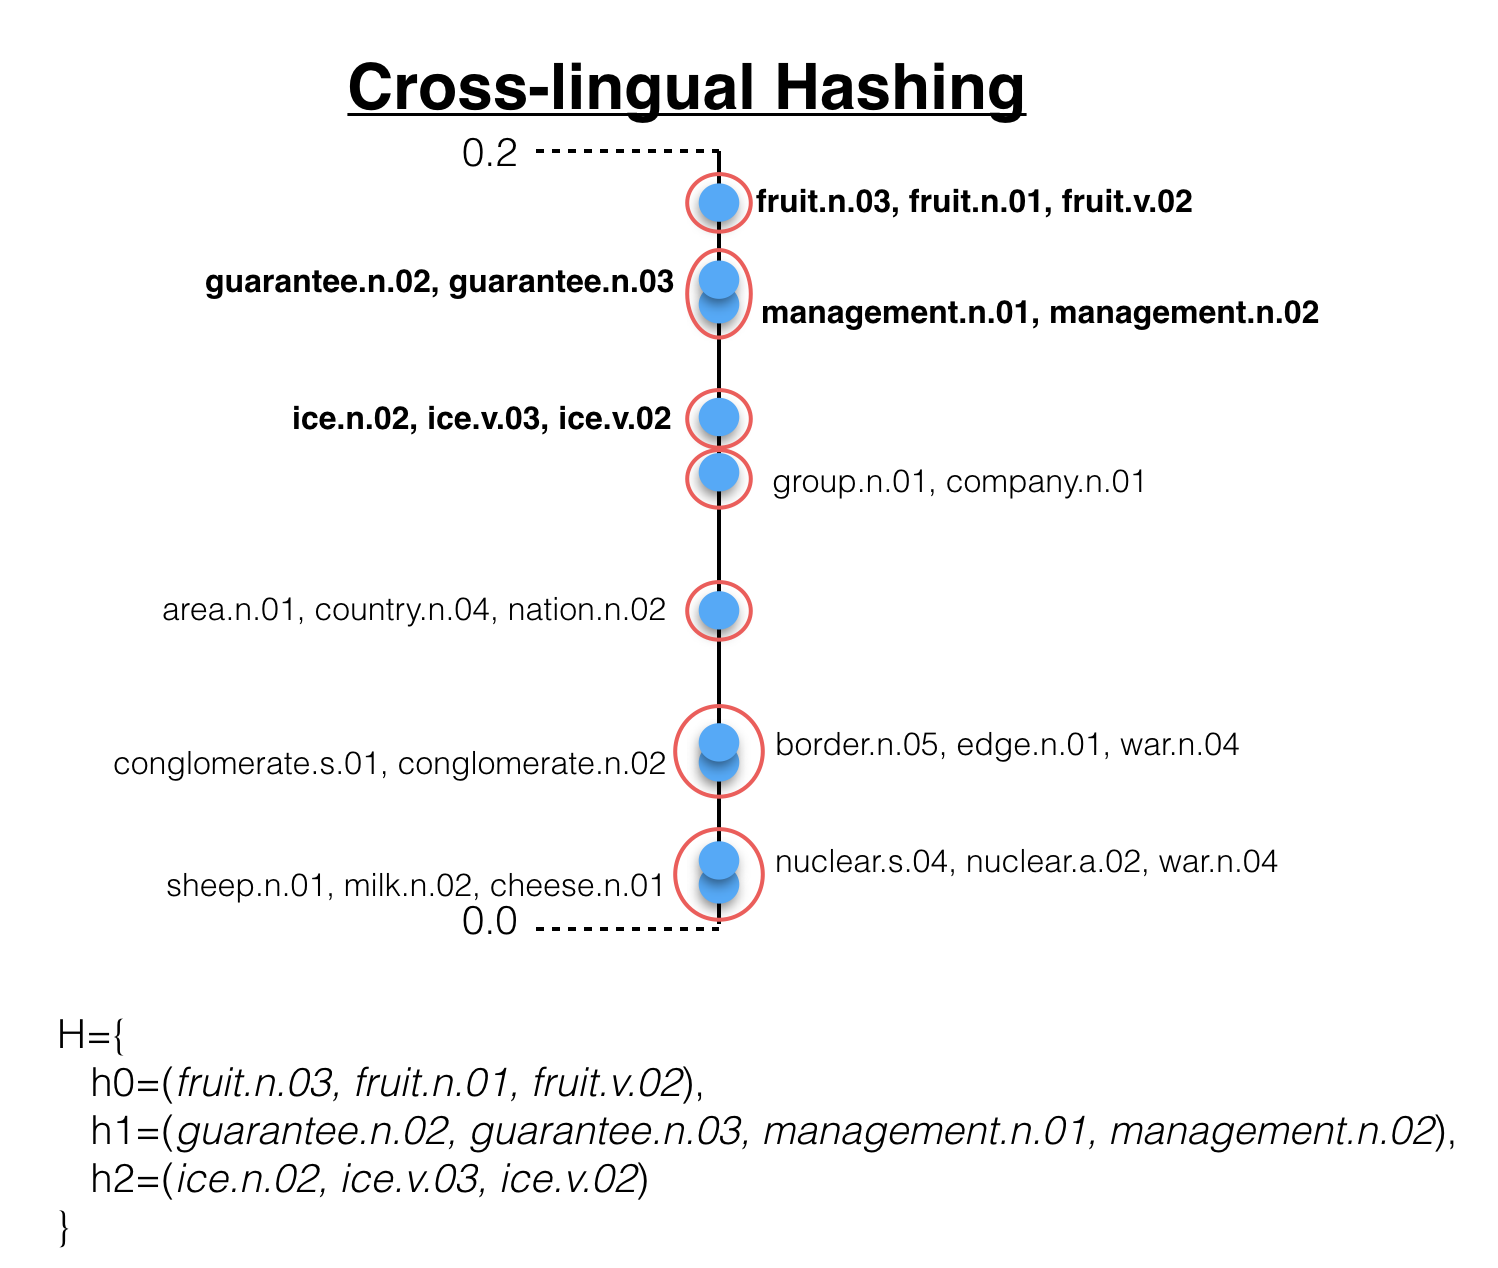
\includegraphics[scale=0.35]{density-hash.png}
\caption{Cross-lingual hash-expression (H) of a document based on WordNet-synset annotations created from the top words of each topic distribution. The most relevant topics are grouped according to their importance in three levels (h0, h1 and h2)}
\label{fig:density_hash2}
\end{figure}


\subsection{Similarity metric}
\label{sec:cl-sim-metric}
In this workspace based on hierarchical representations of topics we use the distance metric proposed in Section \ref{sec:large-distance-metric}, based on the Jaccard coefficient. This metric is mainly used for set-type data \citep{Li2012, Ji2013, Li2010b, Zhao2013} and computes the similarity of sets by looking at the relative size of their intersection (See Eq. \ref{eq:jc}). Thus, it allows us to measure the intersection of cross-lingual topics described by hierarchical hash-sets:

%distance metric formula
\begin{equation}
d_H(H_A,H_B) = \sum\limits_{l=1}^L \Big( d_J(H_A(h_l),H_B(h_l)) \Big) = 
\sum\limits_{l=1}^L \Big( 1 - \frac{H_A(h_l) \cap H_B(h_l)}{H_A(h_l) \cup H_B(h_l)} \Big) 
\label{eq:dh2}
\end{equation}

where $H_A$ and $H_B$ are hash codes, $H_A(h_l)$ and $H_B(h_l)$ are the set of topics up to level $l$ for each hash code $H$,  and $L$ is the maximum hierarchy level. A corner case is $L=T$, where $T$ is the number of topics in the model. 

\subsection{Cross-lingual Models}
\label{sec:crosslingual-models}

\begin{figure*}[ht]\centering
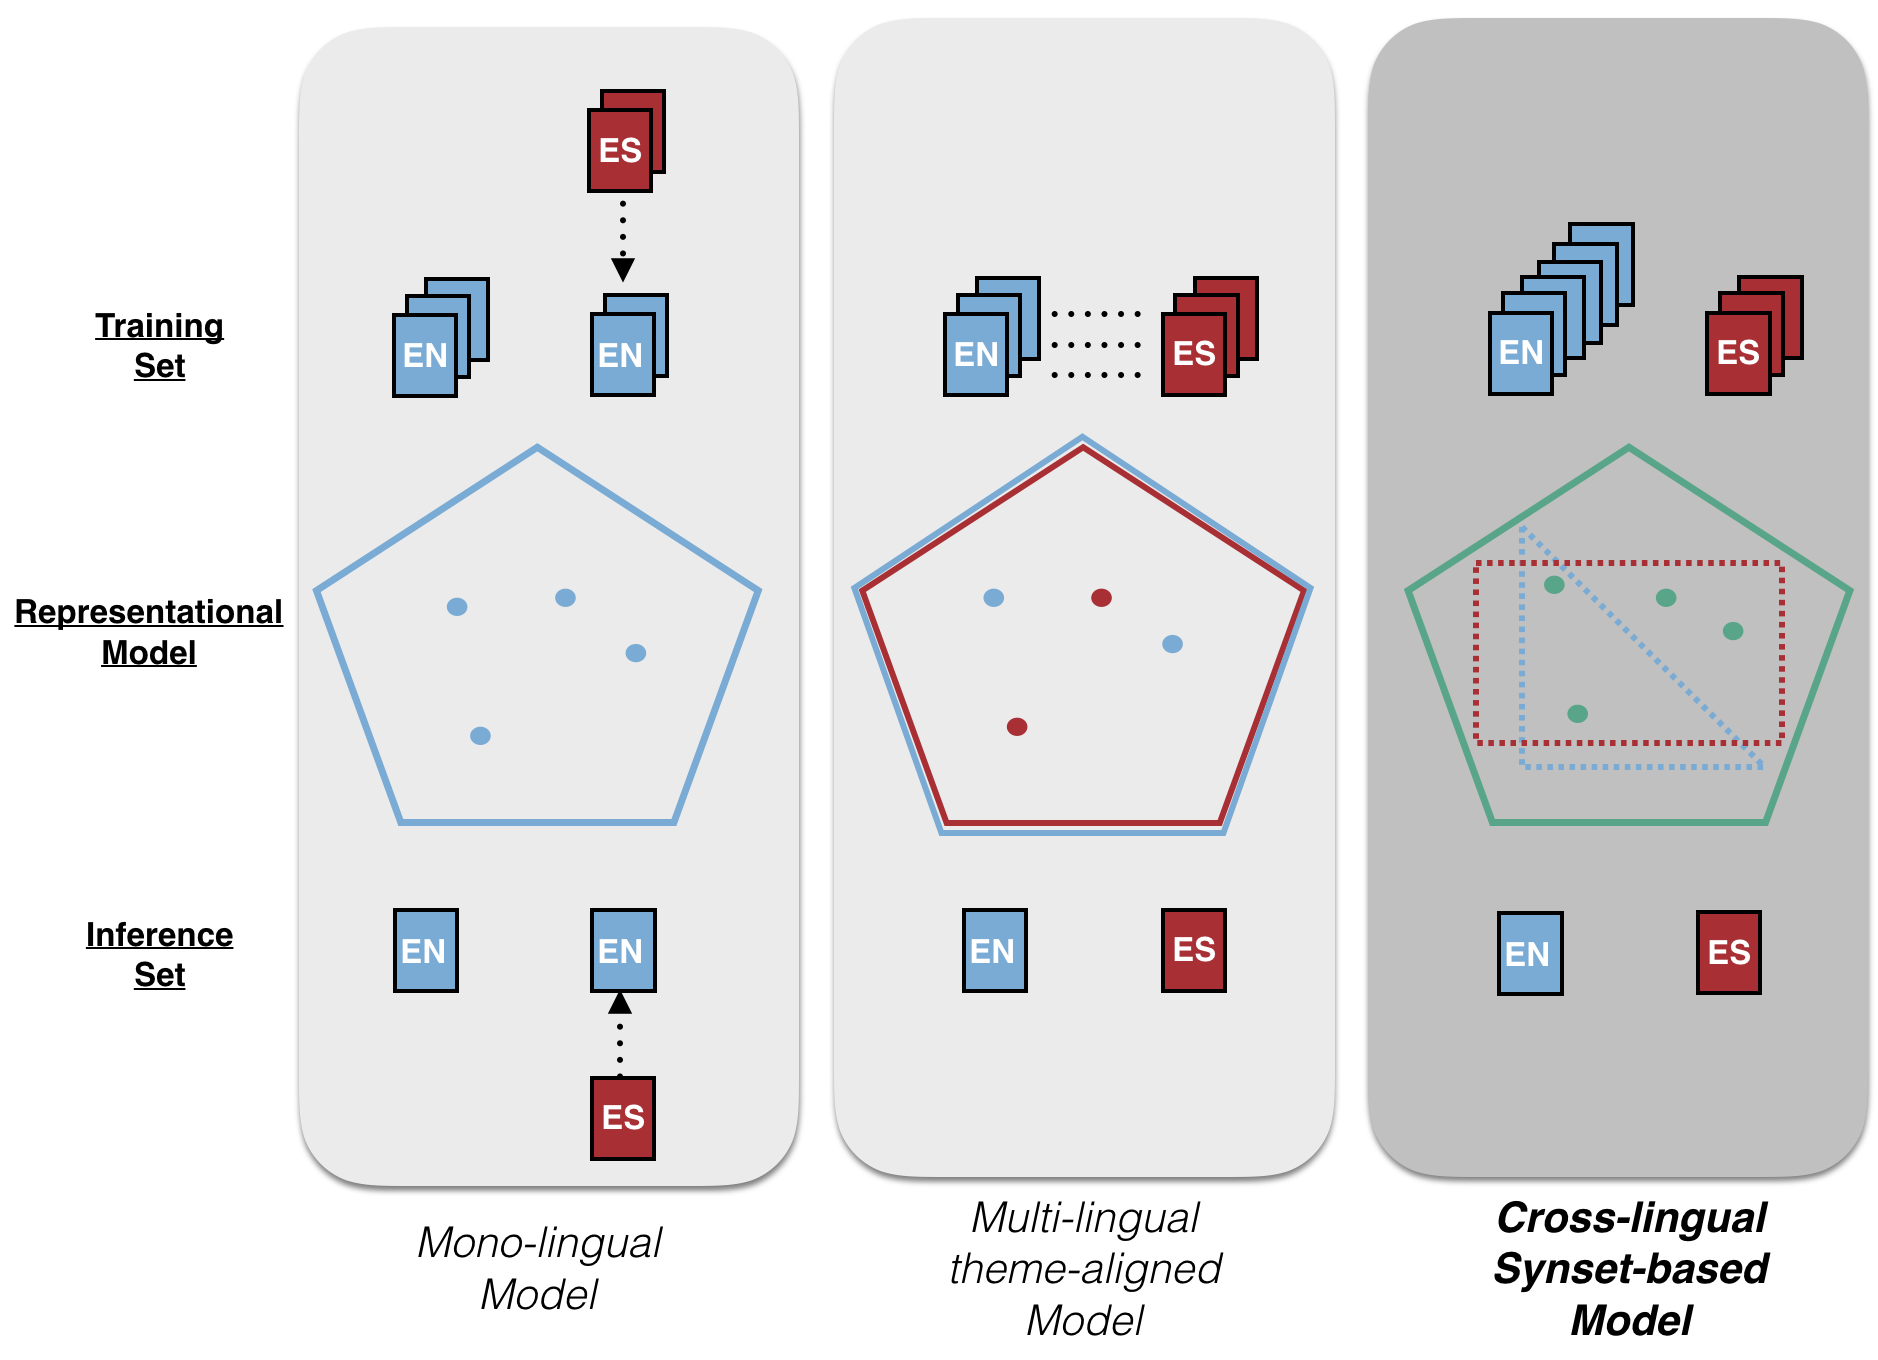
\includegraphics[scale=0.4]{latent-topic-models.png}
\caption{Graphical representation of the model that relies on the latent layer of cross-lingual topics obtained by LDA and hash functions through hierarchies of synsets. Mono-lingual approaches force to translate the documents to the same language to represent them in a unique feature space. Multi-language approaches require previously aligned topics from different languages so that documents can be represented in an equivalent feature space. Cross-lingual Synset-based approach creates a new space by combining the feature spaces of each language (i.e synsets from topn topic words). Documents are then represented in this unique space.}
\label{fig:cross-lingual_topics}
\end{figure*}

Our approach considers that cross-lingual models can be built from non-parallel or even non-comparable collections of multilingual documents. It first creates a probabilistic topic model for each language separately, and then annotates the topics with cross-lingual labels (Fig \ref{fig:cross-lingual_topics}). In the same way, the topic distribution of documents expressed through weighted vectors are first transformed into hierarchies of topics according to their relevance. And then documents are described by a 3-level hierarchy of cross-lingual concepts.

In order to be able to compare the performance of our unsupervised algorithm with a semi-supervised algorithm (MuPTM-based) it is necessary to use theme-aligned corpora that map topics across languages. We used the JRC-Acquis\footnote{https://ec.europa.eu/jrc/en/language-technologies/jrc-acquis} corpora \citep{Steinberger2006}. It is a collection of legislative texts written in 23 languages, although we only use English, Spanish,  French, Italian and Portuguese editions for the tests. Most texts have been manually classified into subject domains according to the EUROVOC\footnote{http://eurovoc.europa.eu/} thesaurus \citep{Eurovoc1995}, which exists in one-to-one translations into approximately twenty languages and distinguishes about 6,000 hierarchically organised descriptors (subject domains). More than 20k documents were used for each language-specific model, a total of 112,569 texts are included in the training-test package, which is publicly available\footnote{http://librairy.linkeddata.es/data/jrc/select?q=*:*} for reuse.

The JRC-Acquis corpus is annotated with EUROVOC categories. These categories are shared among languages and will serve as support for building the topic models. Moreover, the topic independence assumption \citep{Blei2003} of LDA models should be also satisfied, so the categories must first be moved to their base concepts and therefore disjointed categories. The EUROVOC taxonomy has 7,193 concepts/labels from 21 domain areas such as politics, international relations, european union, law, economics, etc. There are 4,904 reciprocal hierarchical relationships (no polyhierarchy) and 6,992 reciprocal associative relationships. Using hierarchical relations, we identified the root concepts from which all other categories derive. The initial 7,193 labels were then reduced to 452 labels, which are independent (topic independence assumption from LDA is satisfied), and can be used to train the topic models. 

\begin{table*}[ht]\centering
  \small
  \noindent
  \begin{tabularx}{\linewidth}{@{} CCCCC @{}}
  \hline
 \textbf{EN-Topic 3} & \textbf{ES-Topic 3} & \textbf{FR-Topic 26} & \textbf{PT-Topic 10} & \textbf{IT-Topic 3}  \\
\textbf{\textit{{\scriptsize "communications systems"}}} & \textbf{\textit{{\scriptsize "sistema de comunicaci\'on"}}} & \textbf{\textit{{\scriptsize "systeme de communication"}}} & \textbf{\textit{{\scriptsize "meios de comunicação"}}} & \textbf{\textit{{\scriptsize "strutture di comunicazione"}}} \\ 
  \hline
     radio          & equipo                & communications		& rede         & rete        \\
     equipment      & red                   & reseaux            & comunicação   & comunicazione        \\
     network        & comunicaci\'on        & electroniques      & electronico    & apparecchiatura        \\
     communication  & espectro              & acces              & acesso    & radio        \\
     regulatory     & electromagn\'etico    & telecommunications & utilizador & regolamentazione            \\
     spectrum       & electr\'onico         & service            & operador & spettro           \\
     electronic     & reglamentaci\'on      & universel          & regulador    & elettronico                  \\
     access         & banda                 & reglamentaires     & universal        & armonizzare        \\
     standard       & etsir                 & nationales         & garantir   & mobile         \\
     mobile         & compatibilidad        & fourniture         & regulamentar  & banda          \\
    \bottomrule
  \end{tabularx}
\caption{Randonly selected theme-aligned topics described by top 10 words based on EUROVOC annotations from JRC-Acquis dataset}
\label{tb:topics}
\end{table*}

 A pre-processing of the documents was required to clean texts and to build a suitable data set for the model. Terms with high frequency are assumed not specific to a particular topic, so words present in more than 90\% of the corpus are considered stopwords and removed from the model. Also, rare terms that occur infrequently are considered not representative of a single topic since they do not appear enough to infer that it is salient for a topic. Then, words present in less than 0.5\% of the corpus are also removed from the model. Lemmatized expressions of names, verbs and adjectives were used to create the bag-of-words, and documents with less than 100 characters were discarded since LDA has proven to have lower performance with these type of texts \citep{Cheng2014a}. 
 
 Then, we set the number of topics $K=500$ (several configurations were evaluated, but this was the closest to the performance obtained with the supervised model based on categories). We run the Gibbs samplers for 1000 training iterations on LDA from our librAIry framework. The Dirichlet priors $\alpha=0.1$ and $\beta=0.01$ were set following \citep{Hu2014a}. Once the word distributions for each topic is available, the list of synsets related with the top5 words for each topic are identified (this number is set to offer better performance after trying several alternatives). Finally, the 3-level hierarchy of topics per document is replaced by a 3-level hierarchy of synsets. Probabilistic topic models in Spanish\footnote{http://librairy.linkeddata.es/jrc-es-model-unsupervised}, English \footnote{http://librairy.linkeddata.es/jrc-en-model-unsupervised}, French\footnote{http://librairy.linkeddata.es/jrc-fr-model-unsupervised}, Italian\footnote{http://librairy.linkeddata.es/jrc-it-model-unsupervised} and Portuguese\footnote{http://librairy.linkeddata.es/jrc-pt-model-unsupervised} were created independently without previously establishing any type of alignment between their topics.
 
 In order to compare the performance of this non-supervised approach with approaches based on aligned topics, we need to use a variant of LDA to force the correspondence between the 452 root categories identified in the EUROVOC thesaurus and the latent topics of the model. Thus, LabeledLDA \citep{Ramage2009a}, a supervised version of LDA, was used to perform parameter estimation. Theme-aligned probabilistic topic models in Spanish\footnote{http://librairy.linkeddata.es/jrc-es-model}, English \footnote{http://librairy.linkeddata.es/jrc-en-model}, French\footnote{http://librairy.linkeddata.es/jrc-fr-model}, Italian \footnote{http://librairy.linkeddata.es/jrc-it-model} and Portuguese \footnote{http://librairy.linkeddata.es/jrc-pt-model} were created sharing the topics but not its definitions (i.e. vocabulary) (see table \ref{tb:topics}).

A simple way of looking at the output quality of the topic models is by simply inspecting top words associated with a particular topic learned during training. A latent topic is semantically coherent if it assigns high probability scores to words that are semantically related \citep{Gliozzo2007, newman-etal-2010-automatic, mimno-etal-2011-optimizing}. It is much easier for humans to judge semantic coherence of cross-lingual topics and their alignment across languages when observing the actual words constituting a topic. These words provide a shallow qualitative representation of the latent topic space, and could be seen as direct and comprehensive word-based summaries of a large document collection.

Samples of cross-lingual topics are provided in Table \ref{tb:topics}. We may consider this visual inspection of the top words associated with each topic as an initial qualitative evaluation, suitable for human judges. Documents present similar topic distributions when projecting their content on topics according to their language as can be seen in fig \ref{fig:topic_distributions}. Since the topic identifiers are not aligned, the graphs appear displaced.

\begin{figure}[ht]\centering
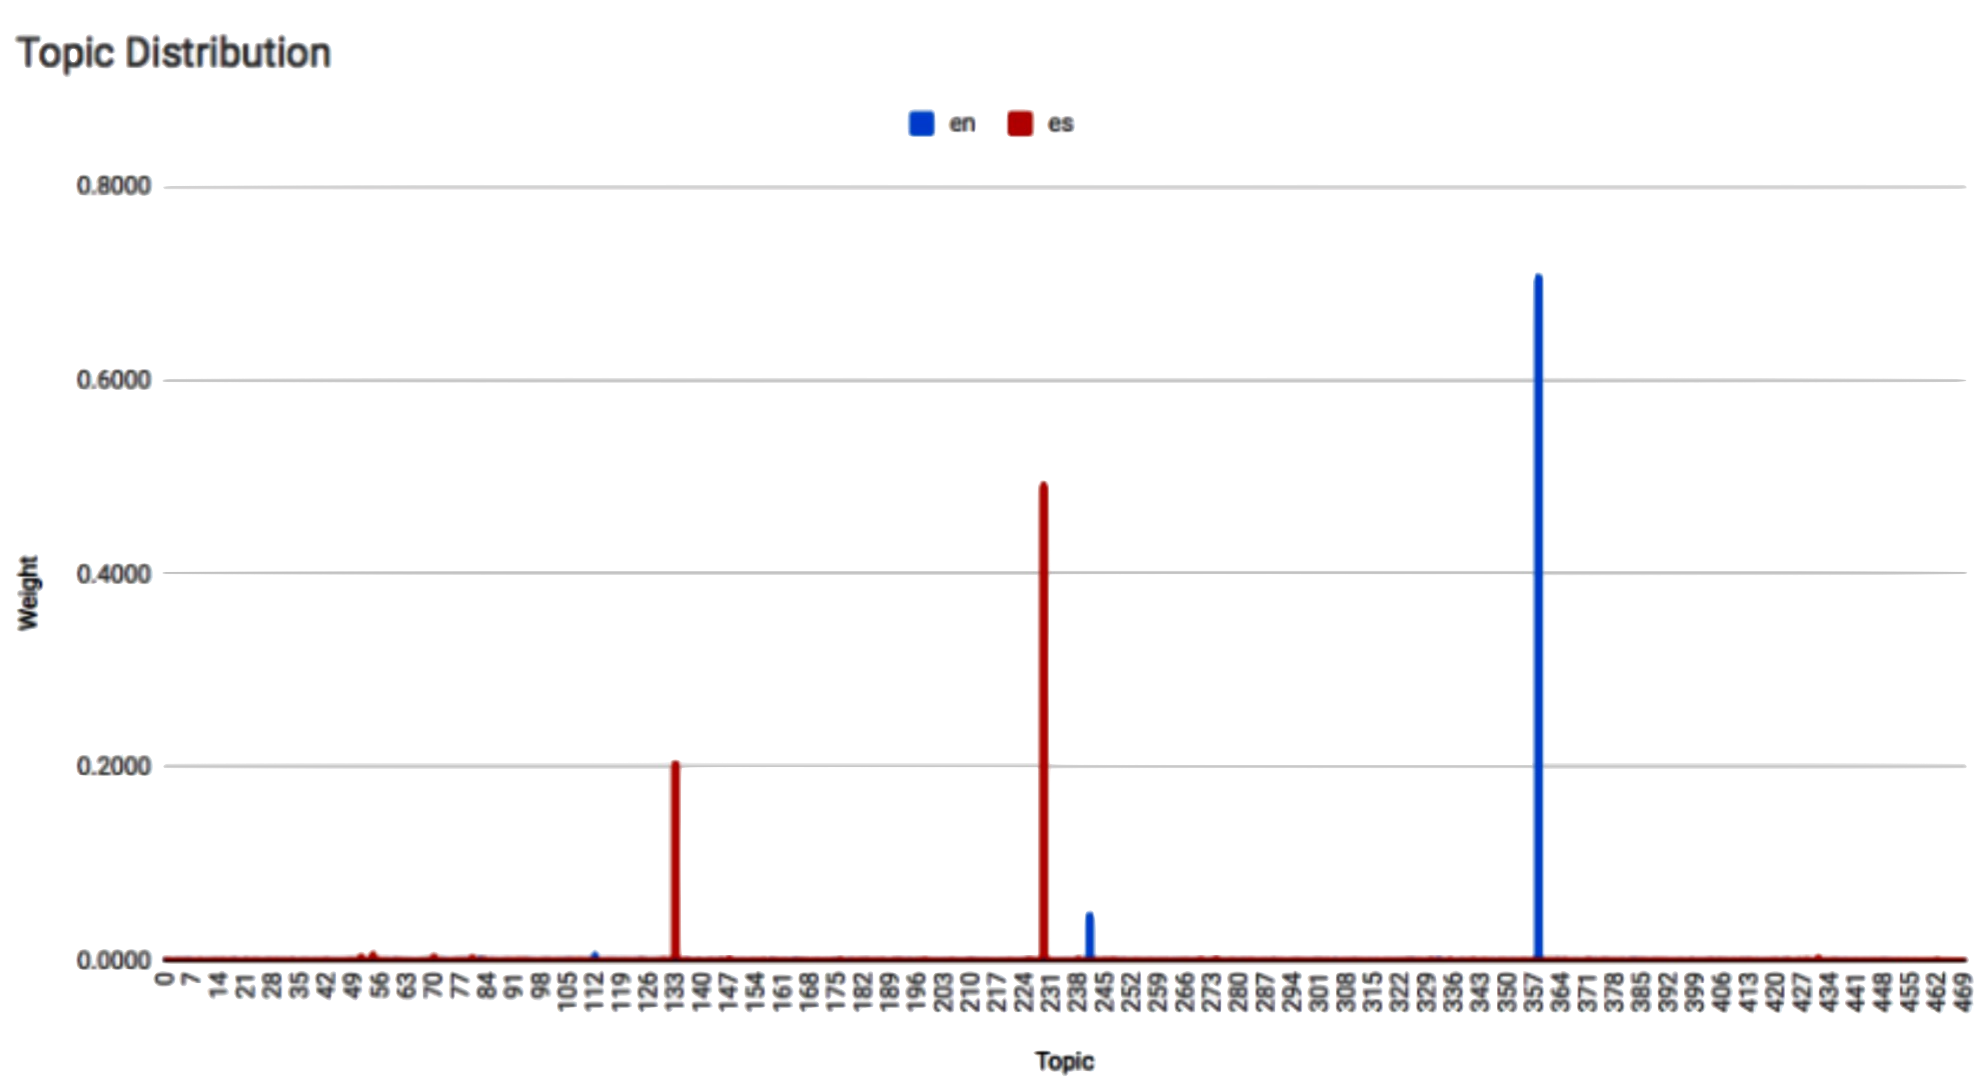
\includegraphics[scale=0.4]{topic-dist.png}
\caption{topic distributions from the same document in English ($h_{EN}=\{(t3062),(t335),(t8278)\}$) and Spanish ($h_{ES}=\{(t335),(t4060),(t5769)\}$).}
\label{fig:topic_distributions}
\end{figure}



\section{Evaluation}
\label{sec:crosslingual-evaluation}

A way to evaluate our cross-lingual document similarity algorithm is to test how well it performs in practice for different real-life tasks: document classification and information retrieval. Evaluation is done using the B-Cubed metrics \citep{Bagga1998} to estimate the fit between two clusters, the one obtained from a supervised category-based topic alignment algorithm and the one obtained from our unsupervised synset-based topic alignment algorithm. 

% table monolingual JRC
\begin{table}[ht]\centering
\begin{center}
\small
\begin{tabular}{cc|rr||rr||rr||rr||rr}
    \hline
    \multicolumn{12}{c}{\textbf{JRC-Acquis Corpora}} \\
    \hline
    & & \multicolumn{2}{c}{\textbf{en}} &
      \multicolumn{2}{c}{\textbf{es}} &
      \multicolumn{2}{c}{\textbf{fr}} &
      \multicolumn{2}{c}{\textbf{pt}} &
      \multicolumn{2}{c}{\textbf{it}}\\
    & & {\textit{cat}} & {\textit{syn}} & {\textit{cat}} & {\textit{syn}} & {\textit{cat}} & {\textit{syn}} & {\textit{cat}} & {\textit{syn}} & {\textit{cat}} & {\textit{syn}} \\
    \hline
    \multirow{4}{*}{\textbf{prec}} 
    &{\textit{min}}     &0.01 &0.01 &0.01 &0.01 &0.01 &0.01 &0.01 &0.01 &0.01 &0.01 \\
    &{\textit{max}}     &1.00 &0.95 &1.00 &0.87 &1.00 &0.87 &1.00 &0.83 &1.00 &0.85\\
    &{\textit{mean}}    &\textbf{0.58} &0.48 &\textbf{0.55} &0.48 &\textbf{0.55} &0.41 &\textbf{0.53} &0.42 &\textbf{0.54} &0.45 \\
    &{\textit{dev}}     &0.27 &0.23 &0.27 &0.22 &0.26 &0.20 &0.24 &0.21 &0.25 &0.22 \\
    \hline
    \multirow{4}{*}{\textbf{rec}} 
    &{\textit{min}}     &0.01 &0.03 &0.01 &0.04 &0.01 &0.05 &0.01 &0.04 &0.01 &0.05\\
    &{\textit{max}}     &0.96 &1.00 &0.93 &1.00 &0.95 &1.00 &0.92 &1.00 &0.94 &1.00\\
    &{\textit{mean}}    &0.39 &\textbf{0.52} &0.36 &\textbf{0.49} &0.42 &\textbf{0.51} &0.40 &\textbf{0.47} &0.39 &\textbf{0.48} \\
    &{\textit{dev}}     &0.24 &0.20 &0.23 &0.20 &0.23 &0.23 &0.23 &0.21 &0.23 &0.20 \\
    \hline
    \multirow{4}{*}{\textbf{f1}} 
    &{\textit{min}}     &0.02 &0.03 &0.01 &0.02 &0.02 &0.03 &0.02 &0.02 &0.01 &0.02 \\
    &{\textit{max}}     &0.70 &0.75 &0.70 &0.71 &0.70 &0.73 &0.70 &0.71 &0.70 &0.72\\
    &{\textit{mean}}    &0.35 &\textbf{0.42} &0.32 &\textbf{0.41} &0.37 &\textbf{0.39} &0.35 &\textbf{0.38} &0.31 &\textbf{0.40} \\
    &{\textit{dev}}     &0.16 &0.15 &0.15 &0.15 &0.17 &0.17 &0.16 &0.16 &0.16 &0.15\\
\end{tabular}
\end{center}
\caption{Document classification performance (precision-'prec', recall-'rec' and fMeasure-'f1') of the categories-based (\textit{cat}) and synset-based (\textit{syn}) topic alignment algorithms in monolingual document collections}
\label{tb:mono-class}
\end{table}


Let $CL_i$ be the cluster that document $t_i$ gets clustered in, and $G_i$ its correct cluster from the ground truth. The B-Cubed metric then calculates $precision=\frac{|CL_i \cap G_i|}{|CL_i|}$ and $recall=\frac{|CL_i \cap G_i|}{|G_i|}$. The total precision and recall of the clustering are taken as the average of the precision and recall scores over all documents. Results are also presented in terms of the $F_1$ measure to balance between precision and recall: $F_1=\frac{2 \cdot precision \cdot recall}{precision + recall}$. The aim is to measure the performance of the algorithm taking into account documents with manual category assignments.

\subsection{Cross-lingual Document Classification}
\label{sec:cl-doc-class}
A random group of 1k documents from the JRC-Acquis corpora, which have not been used to train the models, is considered for evaluation as they are manually tagged with EUROVOC categories. For each document, the cluster to which it belongs is identified from its categories. This cluster is then compared (B-Cubed metrics) with the one obtained from the labels generated from its most representative topics (\textit{cat}) and with the one obtained from the labels generated with the WordNet-Synsets of those topics (\textit{syn}). Algorithm performance is evaluated in monolingual, bilingual, and multilingual document collections (tables \ref{tb:mono-class} and \ref{tb:multi-class} ) .

% table multi-lingual JRC
\begin{table}[ht]\centering
\begin{center}
\small
\begin{tabular}{cc|rr||rr||rr||rr}
    \hline
    \multicolumn{10}{c}{\textbf{JRC-Acquis Corpora}} \\
    \hline
    & & \multicolumn{2}{c}{\textbf{en-es}} &
      \multicolumn{2}{c}{\textbf{en-es-fr}} &
      \multicolumn{2}{c}{\textbf{en-es-fr-pt}} &
      \multicolumn{2}{c}{\textbf{en-es-fr-pt-it}} \\
    & & {\textit{cat}} & {\textit{syn}} & {\textit{cat}} & {\textit{syn}} & {\textit{cat}} & {\textit{syn}} & {\textit{cat}} & {\textit{syn}} \\
    \hline
    \multirow{4}{*}{\textbf{prec}} 
    &{\textit{min}}     &0.01 &0.01 &0.01 &0.01 &0.01 &0.01 &0.01 &0.01\\
    &{\textit{max}}     &1.00 &0.97 &1.00 &0.98 &1.00 &0.97 &1.00 &0.98\\
    &{\textit{mean}}    &\textbf{0.62} &0.55 &\textbf{0.59} &0.52 &\textbf{0.56} &0.50 &\textbf{0.57} &0.52\\
    &{\textit{dev}}     &0.26 &0.23 &0.26 &0.25 &0.26 &0.26 &0.26 &0.26\\
    \hline
    \multirow{4}{*}{\textbf{rec}} 
    &{\textit{min}}     &0.01 &0.09 &0.01 &0.07 &0.01 &0.06 &0.01 &0.04\\
    &{\textit{max}}     &1.00 &1.00 &0.86 &0.93 &0.83 &0.91 &0.80 &0.89\\
    &{\textit{mean}}    &0.33 &\textbf{0.57} &0.25 &\textbf{0.39} &0.21 &\textbf{0.36} &0.23 &\textbf{0.37}\\
    &{\textit{dev}}     &0.16 &0.23 &0.13 &0.15 &0.12 &0.13 &0.12 &0.15\\
    \hline
    \multirow{4}{*}{\textbf{f1}} 
    &{\textit{min}}     &0.02 &0.02 &0.02 &0.05 &0.02 &0.06 &0.02 &0.08\\
    &{\textit{max}}     &0.75 &0.81 &0.62 &0.66 &0.61 &0.64 &0.59 &0.62\\
    &{\textit{mean}}    &0.36 &\textbf{0.49} &0.30 &\textbf{0.38} &0.29 &\textbf{0.35} &0.30 &\textbf{0.36}\\
    &{\textit{dev}}     &0.16 &0.18 &0.11 &0.12 &0.11 &0.11 &0.11 &0.12\\
\end{tabular}
\end{center}
\caption{Document classification performance (precision-'prec', recall-'rec' and fMeasure-'f1') of the categories-based (\textit{cat}) and synset-based (\textit{syn}) topic alignment algorithms in multi-lingual document collections}
\label{tb:multi-class}
\end{table}

The results show a higher performance of the semi-supervised algorithm (categories-based topic alignment) in terms of precision, and of the unsupervised algorithm (synset-based topic alignment) in terms of coverage. The cause lies in the set of synonyms generated by WordNet, being able to share the same synset for two different topics. From a more general point of view (fMeasure), the benefit obtained by the increase in coverage (recall) is greater than by the loss of accuracy (precision).


\subsection{Cross-lingual Information Retrieval}
\label{sec:cl-inf-retrieval}
Given a set of documents and a text, the task is to rank the documents according to their relevance to the query text regardless of the language used. The JRC-Acquis corpus is used because by having texts tagged with EUROVOC categories we can build a ground-truth set grouping the documents that share the same codes as those used in the query document. A collection of 1k randomly selected documents (monolingual, bi-lingual and multi-lingual) are annotated by the category-based and synset-based topic alignment algorithms. Then, we randomly take articles to search in D for documents that share the same categories than the query document (i.e  the ground-truth set). Next, the query text is used to search in D for similar documents using category-based annotations and synset-based annotations. We evaluate the performance of the algorithms in terms of precision@3, precision@5 and precision@10 (tables \ref{tb:mono-ir} and \ref{tb:multi-ir} ) .

% table monolingual TED
\begin{table}[ht]\centering
\begin{center}
\small
\begin{tabular}{cc|rr||rr||rr||rr||rr}
    \hline
    \multicolumn{12}{c}{\textbf{JRC-Acquis Corpora}} \\
    \hline
    & & \multicolumn{2}{c}{\textbf{en}} &
      \multicolumn{2}{c}{\textbf{es}} &
      \multicolumn{2}{c}{\textbf{fr}} &
      \multicolumn{2}{c}{\textbf{pt}} &
      \multicolumn{2}{c}{\textbf{it}} \\
    & & {\textit{cat}} & {\textit{syn}} & {\textit{cat}} & {\textit{syn}} & {\textit{cat}} & {\textit{syn}} & {\textit{cat}} & {\textit{syn}} & {\textit{cat}} & {\textit{syn}} \\
    \hline
    \multirow{2}{*}{\textbf{p@3}} 
    &{\textit{mean}}    &\textbf{0.84} &0.83 &\textbf{0.81} &0.78 &\textbf{0.83} &0.74 &\textbf{0.79} &0.78 &\textbf{0.80} &0.75 \\
    &{\textit{dev}}     &0.26 &0.26 &0.27 &0.29 &0.26 &0.32 &0.27 &0.29 &0.27 &0.29 \\
    \hline
    \multirow{2}{*}{\textbf{p@5}} 
    &{\textit{mean}}    &\textbf{0.82} &0.80 &\textbf{0.79} &0.75 &\textbf{0.80} &0.72 &\textbf{0.77} &0.75 &\textbf{0.78} &0.72 \\
    &{\textit{dev}}     &0.25 &0.25 &0.25 &0.27 &0.25 &0.29 &0.25 &0.26 &0.26 &0.28 \\
    \hline
    \multirow{2}{*}{\textbf{p@10}} 
    &{\textit{mean}}    &\textbf{0.77} &0.76 &\textbf{0.75} &0.73 &\textbf{0.77} &0.68 &\textbf{0.72} &0.71 &\textbf{0.74} &0.68 \\
    &{\textit{dev}}     &0.23 &0.25 &0.25 &0.27 &0.24 &0.27 &0.25 &0.27 &0.25 &0.26 \\
\end{tabular}
\end{center}
\caption{Information retrieval performance (precision@3, precision@5 and precision@10) of the categories-based (\textit{cat}) and synset-based (\textit{syn}) topic alignment algorithms in monolingual document collections}
\label{tb:mono-ir}
\end{table}

% table multi-lingual TED
\begin{table}[ht]\centering
\begin{center}
\small
\begin{tabular}{cc|rr||rr||rr||rr}
    \hline
    \multicolumn{10}{c}{\textbf{JRC-Acquis Corpora}} \\
    \hline
    & & \multicolumn{2}{c}{\textbf{en-es}} &
      \multicolumn{2}{c}{\textbf{en-es-fr}} &
      \multicolumn{2}{c}{\textbf{en-es-fr-pt}} &
      \multicolumn{2}{c}{\textbf{en-es-fr-pt-it}} \\
    & & {\textit{cat}} & {\textit{syn}} & {\textit{cat}} & {\textit{syn}} & {\textit{cat}} & {\textit{syn}} & {\textit{cat}} & {\textit{syn}} \\
    \hline
    \multirow{2}{*}{\textbf{p@3}} 
    &{\textit{mean}}    &\textbf{0.84} &0.79 &\textbf{0.85} &0.75 &\textbf{0.81} &0.69 &\textbf{0.82} &0.71\\
    &{\textit{dev}}     &0.25 &0.28 &0.24 &0.31 &0.23 &0.29 &0.25 &0.29\\
    \hline
    \multirow{2}{*}{\textbf{p@5}} 
    &{\textit{mean}}    &\textbf{0.82} &0.76 &\textbf{0.81} &0.72 &\textbf{0.78} &0.67 &\textbf{0.79} &0.69\\
    &{\textit{dev}}     &0.24 &0.26 &0.23 &0.27 &0.24 &0.25 &0.21 &0.26\\
    \hline
    \multirow{2}{*}{\textbf{p@10}} 
    &{\textit{mean}}    &\textbf{0.78} &0.73 &\textbf{0.76} &0.67 &\textbf{0.73} &0.62 &\textbf{0.74} &0.63\\
    &{\textit{dev}}     &0.22 &0.24 &0.23 &0.26 &0.22 &0.24 &0.23 &0.24\\
\end{tabular}
\end{center}
\caption{Information retrieval performance (precision@3, precision@5 and precision@10) of the categories-based (\textit{cat}) and synset-based (\textit{syn}) topic alignment algorithms in multi-lingual document collections}
\label{tb:multi-ir}
\end{table}

Although the precision values are lower than those obtained by semi-supervised approximation, they are sufficiently promising (around 0.75) to think that introducing improvements in the lemmatization process would increase the quality of the WordNet-synset annotations derived from the most representative words of each topic (precision values close to 0.8 in the English corpus).

\subsection{Text Length on Cross-lingual Representations}

The ability of topics to materialize the underlying knowledge of the documents depend on the texts used to train models. We have studied the impact that the length of texts has, since they determine the space where words can co-occur, to semantically relate multilingual documents described in a probabilistic topic space and, therefore, to capture the knowledge derived from their relationships \citep{Lozano2020}. 

The aim is to know how text length influences the cross-lingual topics created to semantically relate multilingual documents through state-of-the-art similarity metrics (See Chapter \ref{ch:soa}). We have designed several document retrieval tasks based on the models described in Section \ref{sec:crosslingual-models}, to compare the clusters of documents created from their manual annotations (i.e. EUROVOC tags) with those created automatically from their topic distributions (Fig.\ref{fig:workflow}). 

\begin{figure}[ht]
    \centering
    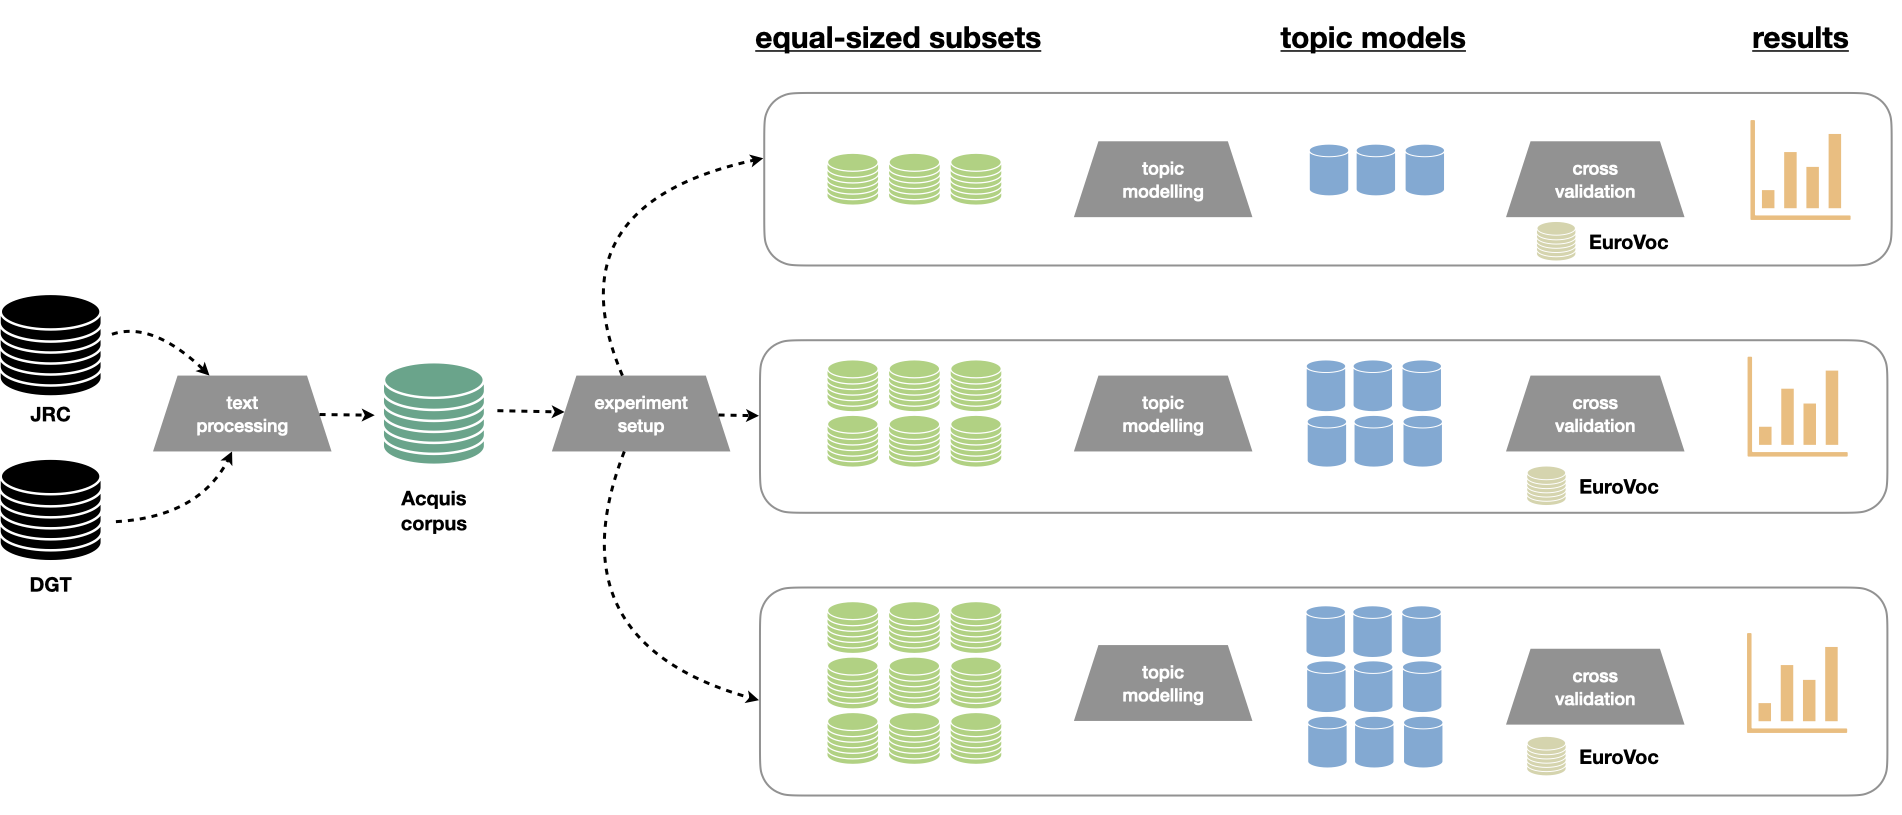
\includegraphics[width=1.0\linewidth]{workflow.png}
    \caption{Preparation of experiments by creating topic models for each \\subset of the original corpus and cross-validated with EuroVoc thesaurus}
    \label{fig:workflow}
\end{figure}


The JRC-Acquis dataset used in the previous experiments (Section \ref{sec:cl-doc-class} and \ref{sec:cl-inf-retrieval}), was extended with the DGT-Acquis \citep{Steinberger2014} collection to increase the total number of documents and the diversity of text length. It contains documents from the Official Journal of the European Union from 2004 to 2011. Given that both datasets are constructed from the same domain with no overlap for data since 2007, we decided to merge both of them into a single collection, the Acquis corpus, formed with all the JRC-Acquis dataset and the documents of DGT-Acquis from that year. \textit{English} and \textit{Spanish} versions of the Acquis corpus were used to validate the results across languages (see table \ref{table:acquis_summ} for a summary of the data used). 

\begin{table}[ht]
\centering
\begin{adjustbox}{max width=0.9\textwidth}
\begin{tabular}{cc|ccc|ccc}
\cline{3-8}
                           &          & \multicolumn{3}{c|}{English}        & \multicolumn{3}{c}{Spanish}         \\ \cline{3-8} 
                           &          & DGT      & JRC      & Acquis   & DGT      & JRC      & Acquis   \\ \hline
\multicolumn{2}{c|}{Documents}      & 51521    & 16260    & 67781    & 51585    & 16470    & 68055    \\ \hline
\multirow{5}{*}{Tokens} & Median   & 135      & 197      & 152      & 129      & 204      & 150      \\
                           & Mean     & 185.8762 & 261.9931 & 204.1359 & 181.9172 & 271.2842 & 203.5449 \\
                           & Variance & 34806.26 & 35716.91 & 36080.66 & 34624.02 & 38700.03 & 37074.97 \\
                           & Min      & 7        & 7        & 7        & 6        & 6        & 6        \\
                           & Max      & 1360     & 1063     & 1360     & 1411     & 1110     & 1411     \\ \hline
\end{tabular}%
\end{adjustbox}
\vspace*{3mm}
\caption{Number of documents and tokens by dataset}
\label{table:acquis_summ}

\end{table}


Texts were pre-processed before the models were trained. We removed stopwords, including general NLP and domain-specific ones based on topic distributions. Rare terms with extremely low total document frequency were also removed. Words were lemmatized and changed to lower-case. A lower and an upper limit on the number of words (i.e. tokens) were defined to discard texts. These bounds were inferred from the interquartile range (Fig. \ref{fig:sizebox}). 


\begin{figure}[ht]\centering
   \begin{minipage}{0.49\textwidth}
     \frame{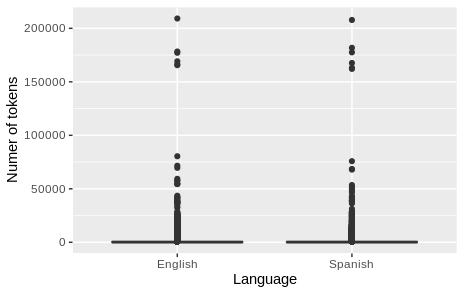
\includegraphics[width=\linewidth]{PreClean.png}}
     \caption{Before pre-processing}\label{subfig:preClean}
   \end{minipage}
   \begin {minipage}[c]{0.49\textwidth}
     \frame{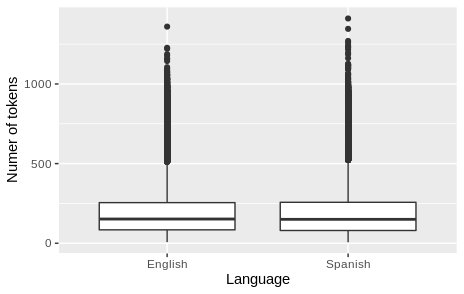
\includegraphics[width=\linewidth]{cleaned.png}}
     \caption{After pre-processing}\label{subfig:postClean}
   \end{minipage}
   \caption{Distribution of articles by number of tokens in corpora}
   \label{fig:sizebox}
\end{figure}


We then divided the original corpora into several subsets (3, 6 and 9) of the same size with texts of similar length. The aim is to compare how similarity metrics based on topic distributions behave for each dataset in document retrieval tasks and to understand the influence of text lengths in the quality of multilingual topic models. For each data set, we reserved a sample ($5\%$) for testing and the rest ($95\%$) was used to train a topic model. The test set was projected in the topic space according to the trained model and then the similarity metrics were used to compare those documents with all documents in the corpus and obtain the most similar ones. The list with the top10 most similar documents is compared in terms of Mean Average Precision (MAP) with the one obtained when comparing them from the EuroVoc labels. This metric allows evaluating on average how good the first 10 results of a query are by taking the mean of all average precision for the first 10 results when comparing a list of retrieved documents and the ground truth.

Each document was manually annotated with one or more EuroVoc categories. Documents that share the same categories were therefore considered semantically related. For each document in the test set, its topic-based similarity to the others is calculated according to density-based metrics (\ref{sec:related-work}) such as Jensen-Shannon divergence (JSD) and Hellinger distance (HE); and our hierarchy-based metric (\ref{sec:large-distance-metric}) that we named Weighted Jaccard Levels (WJL) in experiments. The list of related documents from the EuroVoc categories is then compared to the list of related documents by topics expressed by density or by hierarchies. Since several topic models have been created for each dataset (with 50,100,300 and 500 topics), the precision results for each model were averaged following the mean average precision (MAP) metric. Thus, results reflect the capacity of each topic model to express the knowledge required to relate texts from their content without supervision. Table \ref{table:acquis} shows results for each trained model and each similarity metric. A distinction is made between texts written in English and Spanish. 


\begin{table}[ht]
\centering
\resizebox{0.6\textwidth}{!}{%
\begin{tabular}{ccccc}
\multicolumn{5}{c}{Acquis (MAP@10)}                                                                                                                           \\ \hline
\multicolumn{1}{c|}{Lang}                     & \multicolumn{1}{c|}{Topics} & JSD                               & HE      & WJL                               \\ \hline
\multicolumn{1}{c|}{\multirow{4}{*}{Spanish}} & \multicolumn{1}{c|}{50}     & \textbf{0.80060} & 0.79665 & 0.70583                           \\
\multicolumn{1}{c|}{}                         & \multicolumn{1}{c|}{100}    & \textbf{0.82741} & 0.77930 & 0.75555                           \\
\multicolumn{1}{c|}{}                         & \multicolumn{1}{c|}{300}    & \textbf{0.84261} & 0.58531 & 0.79036                           \\
\multicolumn{1}{c|}{}                         & \multicolumn{1}{c|}{500}    & \textbf{0.81238} & 0.68482 & 0.79336                           \\ \hline
\multicolumn{1}{c|}{\multirow{4}{*}{English}} & \multicolumn{1}{c|}{50}     & \textbf{0.81421} & 0.80150 & 0.73367                           \\
\multicolumn{1}{c|}{}                         & \multicolumn{1}{c|}{100}    & \textbf{0.85510} & 0.74060 & 0.80315                           \\
\multicolumn{1}{c|}{}                         & \multicolumn{1}{c|}{300}    & \textbf{0.84005} & 0.52082 & 0.83277                           \\
\multicolumn{1}{c|}{}                         & \multicolumn{1}{c|}{500}    & 0.78874                           & 0.43636 & \textbf{0.84555} \\ \hline \hline
\end{tabular}%
}
\vspace*{3mm}
\caption{Aggregated MAP results by metric and model}
\label{table:acquis}
\end{table}

The results suggest that PTM highly capture the knowledge required to relate semantically documents, since all models tested had at least one metric above 0.8 in precision. Among the metrics used to relate documents, the Jensen-Shannon divergence (JSD) offers a better performance in general terms compared to the other approaches. Although a downward trend is suggested in density-based metrics when increasing the number of topics, compared to hierarchical metrics that improve their performance when increasing the number of topics. This happens because the sum of distances of the less representative topics for JSD gets bigger as the number of topics diverge from its optimum while activated topics (i.e selected topics at one of the hierarchy levels) get more discriminative which lead to an increase of WJL. Another way to think about the number of topics is the level of detail they capture. Models with low number of topics will present general themes shared by all documents. On the contrary, with more dimensions topics are able to discriminate particular thematics only shared a subset of the document in the collection which is analogous to how EUROVOC and other theasurus works. Hierarchical metrics work best on high-dimensional topic representations because their calculations are based only on the most relevant topics. Therefore, we can conclude that automatically generated annotations from topic models offer a knowledge close to that offered by those manually assigned from the EuroVoc thesaurus in the Acquis legal corpus to relate texts. In the case of large and very heterogeneous collections, i.e. with a high number of different topics, it would be more appropriate to annotate documents by topic hierarchies. In view of these results, the knowledge offered by topics allows automatically discovering what is being treated in a collection of documents, and the knowledge offered by its hierarchical representation allows understanding why documents are related in a similar way as it would be done with manually assigned labels.

\begin{table}[ht]
\centering
\resizebox{0.6\textwidth}{!}{%
\begin{tabular}{ccccccccc}
\multicolumn{9}{c}{Acquis-3 (MAP@10)} \\ \hline
 &  &  & \multicolumn{6}{c}{Training Set} \\ \cline{4-9} 
 &  & \multicolumn{1}{c|}{} & \multicolumn{2}{c|}{1} & \multicolumn{2}{c|}{2} & \multicolumn{2}{c|}{3} \\
 &  & \multicolumn{1}{c|}{} & \textit{es} & \multicolumn{1}{c|}{\textit{en}} & \textit{es} & \multicolumn{1}{c|}{\textit{en}} & \textit{es} & \multicolumn{1}{c|}{\textit{en}} \\ \cline{2-9} 
\multicolumn{1}{c|}{\multirow{6}{*}{\rotatebox[origin=c]{90}{Test Set}}} & \multirow{2}{*}{1} & \multicolumn{1}{c|}{\textit{JSD}} & \cellcolor{gray!25}0.85 & \multicolumn{1}{c|}{\cellcolor{gray!25}0.83} & 0.86 & \multicolumn{1}{c|}{0.85} & \textbf{0.87} & \multicolumn{1}{c|}{\textbf{0.87}} \\
\multicolumn{1}{c|}{} &  & \multicolumn{1}{c|}{\textit{WJL}} & \cellcolor{gray!25}0.85 & \multicolumn{1}{c|}{\cellcolor{gray!25}0.85} & 0.86 & \multicolumn{1}{c|}{0.86} & 0.85 & \multicolumn{1}{c|}{0.86} \\ \cline{2-9} 
\multicolumn{1}{c|}{} & \multirow{2}{*}{2} & \multicolumn{1}{c|}{\textit{JSD}} & 0.80 & \multicolumn{1}{c|}{0.75} & \cellcolor{gray!25}0.77 & \multicolumn{1}{c|}{\cellcolor{gray!25}0.75} & \textbf{0.82} & \multicolumn{1}{c|}{0.80} \\
\multicolumn{1}{c|}{} &  & \multicolumn{1}{c|}{\textit{WJL}} & 0.73 & \multicolumn{1}{c|}{0.77} & \cellcolor{gray!25}0.81 & \multicolumn{1}{c|}{\cellcolor{gray!25}0.83} & 0.82 & \multicolumn{1}{c|}{\textbf{0.83}} \\ \cline{2-9} 
\multicolumn{1}{c|}{} & \multirow{2}{*}{3} & \multicolumn{1}{c|}{\textit{JSD}} & 0.72 & \multicolumn{1}{c|}{0.62} & 0.68 & \multicolumn{1}{c|}{0.65} & \cellcolor{gray!25}0.69 & \multicolumn{1}{c|}{\cellcolor{gray!25}0.68} \\
\multicolumn{1}{c|}{} &  & \multicolumn{1}{c|}{\textit{WJL}} & 0.55 & \multicolumn{1}{c|}{0.65} & 0.67 & \multicolumn{1}{c|}{0.72} & \textbf{\cellcolor{gray!25}0.73} & \multicolumn{1}{c|}{\textbf{\cellcolor{gray!25}0.77}} \\ \cline{2-9} 
\end{tabular}%
 }
 \vspace*{3mm}
 \caption{MAP results by dividing the corpus into three equal subsets to train and evaluate the models in English(\textit{en}) and Spanish(\textit{es})}
 \label{table:acquis3}
\end{table}


To better understand how the length of the texts affects the creation of probabilistic topics, we have prepared three different scenarios that divided the original corpora into subsets with similar text sizes. In the first scenario we have created three equal sets (Table \ref{table:acquis3}), in the second scenario there were six subsets (Table \ref{table:acquis6}), and in the third scenario a total of nine subsets were created (Table \ref{table:acquis9}). We have only considered the similarities calculated from JSD and WJL, as they offered the best performance for each approach.

\begin{table}[ht]
\makebox[\textwidth][c]{
\resizebox{0.85\textwidth}{!}{%
\begin{tabular}{ccccccccccccccc}
\multicolumn{15}{c}{Acquis-6 (MAP@10)} \\ \hline
 &  & \textit{} & \multicolumn{12}{c}{Training Set} \\ \cline{4-15} 
 &  & \multicolumn{1}{c|}{\textit{}} & \multicolumn{2}{c|}{1} & \multicolumn{2}{c|}{2} & \multicolumn{2}{c|}{3} & \multicolumn{2}{c|}{4} & \multicolumn{2}{c|}{5} & \multicolumn{2}{c|}{6} \\
\textit{} & \textit{} & \multicolumn{1}{c|}{} & \textit{es} & \multicolumn{1}{c|}{\textit{en}} & \textit{es} & \multicolumn{1}{c|}{\textit{en}} & \textit{es} & \multicolumn{1}{c|}{\textit{en}} & \textit{es} & \multicolumn{1}{c|}{\textit{en}} & \textit{es} & \multicolumn{1}{c|}{\textit{en}} & \textit{es} & \multicolumn{1}{c|}{\textit{en}} \\ \cline{2-15} 
\multicolumn{1}{c|}{\multirow{12}{*}{\rotatebox[origin=c]{90}{Test Set}}} & \multirow{2}{*}{1} & \multicolumn{1}{c|}{\textit{jsd}} & \cellcolor{gray!25}0.79 & \multicolumn{1}{c|}{\cellcolor{gray!25}0.76} & 0.79 & \multicolumn{1}{c|}{0.77} & 0.79 & \multicolumn{1}{c|}{\textbf{0.78}} & \textbf{0.79} & \multicolumn{1}{c|}{0.77} & 0.79 & \multicolumn{1}{c|}{0.77} & 0.77 & \multicolumn{1}{c|}{0.73} \\
\multicolumn{1}{c|}{} &  & \multicolumn{1}{c|}{\textit{wjl}} & \cellcolor{gray!25}0.78 & \multicolumn{1}{c|}{\cellcolor{gray!25}0.74} & 0.78 & \multicolumn{1}{c|}{0.76} & 0.77 & \multicolumn{1}{c|}{0.77} & 0.78 & \multicolumn{1}{c|}{0.76} & 0.78 & \multicolumn{1}{c|}{0.76} & 0.74 & \multicolumn{1}{c|}{0.69} \\ \cline{2-15} 
\multicolumn{1}{c|}{} & \multirow{2}{*}{2} & \multicolumn{1}{c|}{\textit{jsd}} & 0.82 & \multicolumn{1}{c|}{0.80} & \cellcolor{gray!25}0.81 & \multicolumn{1}{c|}{\cellcolor{gray!25}0.77} & 0.80 & \multicolumn{1}{c|}{0.76} & 0.81 & \multicolumn{1}{c|}{0.79} & 0.85 & \multicolumn{1}{c|}{0.82} & 0.84 & \multicolumn{1}{c|}{0.84} \\
\multicolumn{1}{c|}{} &  & \multicolumn{1}{c|}{\textit{wjl}} & 0.81 & \multicolumn{1}{c|}{0.82} & \cellcolor{gray!25}\textbf{0.85} & \multicolumn{1}{c|}{\cellcolor{gray!25}0.86} & 0.84 & \multicolumn{1}{c|}{\textbf{0.86}} & 0.85 & \multicolumn{1}{c|}{0.85} & 0.85 & \multicolumn{1}{c|}{0.85} & 0.83 & \multicolumn{1}{c|}{0.84} \\ \cline{2-15} 
\multicolumn{1}{c|}{} & \multirow{2}{*}{3} & \multicolumn{1}{c|}{\textit{jsd}} & 0.76 & \multicolumn{1}{c|}{0.73} & 0.78 & \multicolumn{1}{c|}{0.73} & \cellcolor{gray!25}0.72 & \multicolumn{1}{c|}{\cellcolor{gray!25}0.68} & 0.78 & \multicolumn{1}{c|}{0.71} & 0.81 & \multicolumn{1}{c|}{0.75} & 0.81 & \multicolumn{1}{c|}{0.76} \\
\multicolumn{1}{c|}{} &  & \multicolumn{1}{c|}{\textit{wjl}} & 0.73 & \multicolumn{1}{c|}{0.70} & 0.72 & \multicolumn{1}{c|}{0.78} & \cellcolor{gray!25}0.81 & \multicolumn{1}{c|}{\cellcolor{gray!25}0.79} & 0.81 & \multicolumn{1}{c|}{0.80} & \textbf{0.82} & \multicolumn{1}{c|}{\textbf{0.80}} & 0.79 & \multicolumn{1}{c|}{0.80} \\ \cline{2-15} 
\multicolumn{1}{c|}{} & \multirow{2}{*}{4} & \multicolumn{1}{c|}{\textit{jsd}} & 0.69 & \multicolumn{1}{c|}{0.68} & 0.72 & \multicolumn{1}{c|}{0.67} & 0.71 & \multicolumn{1}{c|}{0.68} & \cellcolor{gray!25}0.68 & \multicolumn{1}{c|}{\cellcolor{gray!25}0.63} & 0.73 & \multicolumn{1}{c|}{0.69} & 0.74 & \multicolumn{1}{c|}{0.71} \\
\multicolumn{1}{c|}{} &  & \multicolumn{1}{c|}{\textit{wjl}} & 0.63 & \multicolumn{1}{c|}{0.69} & 0.66 & \multicolumn{1}{c|}{0.72} & 0.74 & \multicolumn{1}{c|}{0.76} & \cellcolor{gray!25}0.77 & \multicolumn{1}{c|}{\cellcolor{gray!25}0.78} & \textbf{0.77} & \multicolumn{1}{c|}{\textbf{0.79}} & 0.75 & \multicolumn{1}{c|}{\textbf{0.79}} \\ \cline{2-15} 
\multicolumn{1}{c|}{} & \multirow{2}{*}{5} & \multicolumn{1}{c|}{\textit{jsd}} & 0.62 & \multicolumn{1}{c|}{0.57} & 0.69 & \multicolumn{1}{c|}{0.61} & 0.66 & \multicolumn{1}{c|}{0.62} & 0.67 & \multicolumn{1}{c|}{0.59} & \cellcolor{gray!25}0.63 & \multicolumn{1}{c|}{\cellcolor{gray!25}0.59} & 0.70 & \multicolumn{1}{c|}{0.65} \\
\multicolumn{1}{c|}{} &  & \multicolumn{1}{c|}{\textit{wjl}} & 0.60 & \multicolumn{1}{c|}{0.63} & 0.57 & \multicolumn{1}{c|}{0.64} & 0.65 & \multicolumn{1}{c|}{0.69} & 0.70 & \multicolumn{1}{c|}{0.71} & \cellcolor{gray!25}\textbf{0.73} & \multicolumn{1}{c|}{\cellcolor{gray!25}0.74} & 0.72 & \multicolumn{1}{c|}{\textbf{0.75}} \\ \cline{2-15} 
\multicolumn{1}{c|}{} & \multirow{2}{*}{6} & \multicolumn{1}{c|}{\textit{jsd}} & 0.55 & \multicolumn{1}{c|}{0.52} & 0.67 & \multicolumn{1}{c|}{0.56} & 0.61 & \multicolumn{1}{c|}{0.56} & 0.63 & \multicolumn{1}{c|}{0.56} & 0.63 & \multicolumn{1}{c|}{0.56} & \cellcolor{gray!25}0.59 & \multicolumn{1}{c|}{\cellcolor{gray!25}0.55} \\
\multicolumn{1}{c|}{} &  & \multicolumn{1}{c|}{\textit{wjl}} & 0.51 & \multicolumn{1}{c|}{0.57} & 0.51 & \multicolumn{1}{c|}{0.60} & 0.58 & \multicolumn{1}{c|}{0.63} & 0.63 & \multicolumn{1}{c|}{0.67} & 0.66 & \multicolumn{1}{c|}{0.70} & \cellcolor{gray!25}\textbf{0.69} & \multicolumn{1}{c|}{\cellcolor{gray!25}\textbf{0.71}} \\ \cline{2-15} 
\end{tabular}%
}}
 \vspace*{3mm}
\caption{MAP results by dividing the corpus into six equal subsets to train and evaluate the models in English(\textit{en}) and Spanish(\textit{es})} 
 \label{table:acquis6}
\end{table}


Models created from texts (training set) with greater or equal length to the texts used in the inferences (test set) offered better performance in document retrieval tasks regardless of the language used. This is evidenced by the fact that those models performed better for almost all sets. Although for some evaluations of small documents models trained with large texts didn't yield the best performances they were not significantly different from the best models. For small documents both metrics performed similarly. 

\begin{table}[ht]

\makebox[\textwidth][c]{
\resizebox{1.0\textwidth}{!}{%
\begin{tabular}{ccccccccccccccccccccc}
\multicolumn{21}{c}{Acquis-9 (MAP@10)} \\ \hline
 &  & \textit{} & \multicolumn{18}{c}{Training Set} \\ \cline{4-21} 
 &  & \multicolumn{1}{c|}{\textit{}} & \multicolumn{2}{c|}{1} & \multicolumn{2}{c|}{2} & \multicolumn{2}{c|}{3} & \multicolumn{2}{c|}{4} & \multicolumn{2}{c|}{5} & \multicolumn{2}{c|}{6} & \multicolumn{2}{c|}{7} & \multicolumn{2}{c|}{8} & \multicolumn{2}{c|}{9} \\
\textit{} & \textit{} & \multicolumn{1}{c|}{} & \textit{es} & \multicolumn{1}{c|}{\textit{en}} & \textit{es} & \multicolumn{1}{c|}{\textit{en}} & \textit{es} & \multicolumn{1}{c|}{\textit{en}} & \textit{es} & \multicolumn{1}{c|}{\textit{en}} & \textit{es} & \multicolumn{1}{c|}{\textit{en}} & \textit{es} & \multicolumn{1}{c|}{\textit{en}} & \textit{es} & \multicolumn{1}{c|}{\textit{en}} & \textit{es} & \multicolumn{1}{c|}{\textit{en}} & \textit{es} & \multicolumn{1}{c|}{\textit{en}} \\ \cline{2-21} 
\multicolumn{1}{c|}{\multirow{18}{*}{\rotatebox[origin=c]{90}{Test Set}}} & \multirow{2}{*}{1} & \multicolumn{1}{c|}{\textit{jsd}} & \cellcolor{gray!25}0.88 & \multicolumn{1}{c|}{\cellcolor{gray!25}0.85} & 0.87 & \multicolumn{1}{c|}{0.87} & 0.88 & \multicolumn{1}{c|}{0.88} & 0.88 & \multicolumn{1}{c|}{0.8} & 0.89 & \multicolumn{1}{c|}{0.89} & 0.88 & \multicolumn{1}{c|}{0.88} & 0.89 & \multicolumn{1}{c|}{\textbf{0.89}} & \textbf{0.89} & \multicolumn{1}{c|}{0.88} & 0.88 & \multicolumn{1}{c|}{0.82} \\
\multicolumn{1}{c|}{} &  & \multicolumn{1}{c|}{\textit{wjl}} & \cellcolor{gray!25}0.89 & \multicolumn{1}{c|}{\cellcolor{gray!25}0.79} & 0.89 & \multicolumn{1}{c|}{0.82} & 0.87 & \multicolumn{1}{c|}{0.86} & 0.88 & \multicolumn{1}{c|}{0.86} & 0.89 & \multicolumn{1}{c|}{0.87} & 0.88 & \multicolumn{1}{c|}{0.87} & 0.89 & \multicolumn{1}{c|}{0.87} & 0.89 & \multicolumn{1}{c|}{0.87} & 0.87 & \multicolumn{1}{c|}{0.77} \\ \cline{2-21} 
\multicolumn{1}{c|}{} & \multirow{2}{*}{2} & \multicolumn{1}{c|}{\textit{jsd}} & 0.70 & \multicolumn{1}{c|}{0.66} & \cellcolor{gray!25}0.70 & \multicolumn{1}{c|}{\cellcolor{gray!25}0.63} & 0.71 & \multicolumn{1}{c|}{0.64} & 0.69 & \multicolumn{1}{c|}{0.63} & 0.71 & \multicolumn{1}{c|}{0.66} & 0.72 & \multicolumn{1}{c|}{0.68} & 0.73 & \multicolumn{1}{c|}{0.70} & \textbf{0.74} & \multicolumn{1}{c|}{\textbf{0.73}} & 0.71 & \multicolumn{1}{c|}{0.71} \\
\multicolumn{1}{c|}{} &  & \multicolumn{1}{c|}{\textit{wjl}} & 0.64 & \multicolumn{1}{c|}{0.59} & \cellcolor{gray!25}0.69 & \multicolumn{1}{c|}{\cellcolor{gray!25}0.69} & 0.69 & \multicolumn{1}{c|}{0.70} & 0.71 & \multicolumn{1}{c|}{0.68} & 0.69 & \multicolumn{1}{c|}{0.69} & 0.71 & \multicolumn{1}{c|}{0.69} & 0.71 & \multicolumn{1}{c|}{0.70} & 0.72 & \multicolumn{1}{c|}{0.71} & 0.67 & \multicolumn{1}{c|}{0.68} \\ \cline{2-21} 
\multicolumn{1}{c|}{} & \multirow{2}{*}{3} & \multicolumn{1}{c|}{\textit{jsd}} & 0.83 & \multicolumn{1}{c|}{0.82} & 0.86 & \multicolumn{1}{c|}{0.80} & \cellcolor{gray!25}0.80 & \multicolumn{1}{c|}{\cellcolor{gray!25}0.75} & 0.81 & \multicolumn{1}{c|}{0.75} & 0.83 & \multicolumn{1}{c|}{0.77} & 0.83 & \multicolumn{1}{c|}{0.79} & 0.85 & \multicolumn{1}{c|}{0.81} & 0.86 & \multicolumn{1}{c|}{0.81} & 0.84 & \multicolumn{1}{c|}{0.82} \\
\multicolumn{1}{c|}{} &  & \multicolumn{1}{c|}{\textit{wjl}} & 0.80 & \multicolumn{1}{c|}{0.78} & 0.84 & \multicolumn{1}{c|}{0.83} & \cellcolor{gray!25}0.87 & \multicolumn{1}{c|}{\cellcolor{gray!25}0.86} & \textbf{0.88} & \multicolumn{1}{c|}{\textbf{0.86}} & 0.88 & \multicolumn{1}{c|}{0.85} & 0.87 & \multicolumn{1}{c|}{0.85} & 0.86 & \multicolumn{1}{c|}{0.85} & 0.87 & \multicolumn{1}{c|}{0.84} & 0.84 & \multicolumn{1}{c|}{0.83} \\ \cline{2-21} 
\multicolumn{1}{c|}{} & \multirow{2}{*}{4} & \multicolumn{1}{c|}{\textit{jsd}} & 0.74 & \multicolumn{1}{c|}{0.72} & 0.77 & \multicolumn{1}{c|}{0.70} & 0.72 & \multicolumn{1}{c|}{0.67} & \cellcolor{gray!25}0.65 & \multicolumn{1}{c|}{\cellcolor{gray!25}0.63} & 0.69 & \multicolumn{1}{c|}{0.63} & 0.73 & \multicolumn{1}{c|}{0.66} & 0.76 & \multicolumn{1}{c|}{0.70} & 0.78 & \multicolumn{1}{c|}{0.72} & 0.77 & \multicolumn{1}{c|}{0.73} \\
\multicolumn{1}{c|}{} &  & \multicolumn{1}{c|}{\textit{wjl}} & 0.68 & \multicolumn{1}{c|}{0.67} & 0.73 & \multicolumn{1}{c|}{0.73} & 0.76 & \multicolumn{1}{c|}{0.77} & \cellcolor{gray!25}0.78 & \multicolumn{1}{c|}{\cellcolor{gray!25}\textbf{0.80}} & 0.79 & \multicolumn{1}{c|}{0.78} & \textbf{0.80} & \multicolumn{1}{c|}{0.79} & 0.80 & \multicolumn{1}{c|}{0.79} & 0.80 & \multicolumn{1}{c|}{0.77} & 0.77 & \multicolumn{1}{c|}{0.76} \\ \cline{2-21} 
\multicolumn{1}{c|}{} & \multirow{2}{*}{5} & \multicolumn{1}{c|}{\textit{jsd}} & 0.68 & \multicolumn{1}{c|}{0.68} & 0.73 & \multicolumn{1}{c|}{0.67} & 0.70 & \multicolumn{1}{c|}{0.66} & 0.68 & \multicolumn{1}{c|}{0.64} & \cellcolor{gray!25}0.62 & \multicolumn{1}{c|}{\cellcolor{gray!25}0.59} & 0.69 & \multicolumn{1}{c|}{0.62} & 0.71 & \multicolumn{1}{c|}{0.67} & 0.73 & \multicolumn{1}{c|}{0.67} & 0.74 & \multicolumn{1}{c|}{0.70} \\
\multicolumn{1}{c|}{} &  & \multicolumn{1}{c|}{\textit{wjl}} & 0.60 & \multicolumn{1}{c|}{0.65} & 0.64 & \multicolumn{1}{c|}{0.72} & 0.67 & \multicolumn{1}{c|}{0.73} & 0.72 & \multicolumn{1}{c|}{0.76} & \cellcolor{gray!25}0.75 & \multicolumn{1}{c|}{\cellcolor{gray!25}0.77} & \textbf{0.77} & \multicolumn{1}{c|}{\textbf{0.78}} & 0.73 & \multicolumn{1}{c|}{0.78} & 0.75 & \multicolumn{1}{c|}{0.77} & 0.74 & \multicolumn{1}{c|}{0.77} \\ \cline{2-21} 
\multicolumn{1}{c|}{} & \multirow{2}{*}{6} & \multicolumn{1}{c|}{\textit{jsd}} & 0.61 & \multicolumn{1}{c|}{0.61} & 0.68 & \multicolumn{1}{c|}{0.59} & 0.64 & \multicolumn{1}{c|}{0.58} & 0.63 & \multicolumn{1}{c|}{0.59} & 0.63 & \multicolumn{1}{c|}{0.56} & \cellcolor{gray!25}0.57 & \multicolumn{1}{c|}{\cellcolor{gray!25}0.54} & 0.65 & \multicolumn{1}{c|}{0.59} & 0.68 & \multicolumn{1}{c|}{0.60} & 0.68 & \multicolumn{1}{c|}{0.62} \\
\multicolumn{1}{c|}{} &  & \multicolumn{1}{c|}{\textit{wjl}} & 0.53 & \multicolumn{1}{c|}{0.58} & 0.61 & \multicolumn{1}{c|}{0.65} & 0.60 & \multicolumn{1}{c|}{0.65} & 0.67 & \multicolumn{1}{c|}{0.70} & 0.69 & \multicolumn{1}{c|}{0.71} & \cellcolor{gray!25}0.69 & \multicolumn{1}{c|}{\cellcolor{gray!25}0.73} & 0.71 & \multicolumn{1}{c|}{0.73} & \textbf{0.71} & \multicolumn{1}{c|}{\textbf{0.74}} & 0.69 & \multicolumn{1}{c|}{0.71} \\ \cline{2-21} 
\multicolumn{1}{c|}{} & \multirow{2}{*}{7} & \multicolumn{1}{c|}{\textit{jsd}} & 0.53 & \multicolumn{1}{c|}{0.57} & 0.62 & \multicolumn{1}{c|}{0.52} & 0.59 & \multicolumn{1}{c|}{0.53} & 0.56 & \multicolumn{1}{c|}{0.54} & 0.58 & \multicolumn{1}{c|}{0.52} & 0.57 & \multicolumn{1}{c|}{0.52} & \cellcolor{gray!25}0.52 & \multicolumn{1}{c|}{\cellcolor{gray!25}0.50} & 0.59 & \multicolumn{1}{c|}{0.53} & 0.63 & \multicolumn{1}{c|}{0.55} \\
\multicolumn{1}{c|}{} &  & \multicolumn{1}{c|}{\textit{wjl}} & 0.47 & \multicolumn{1}{c|}{0.55} & 0.53 & \multicolumn{1}{c|}{0.63} & 0.52 & \multicolumn{1}{c|}{0.64} & 0.58 & \multicolumn{1}{c|}{0.66} & 0.62 & \multicolumn{1}{c|}{0.66} & 0.65 & \multicolumn{1}{c|}{0.69} & \cellcolor{gray!25}0.65 & \multicolumn{1}{c|}{\cellcolor{gray!25}0.70} & \textbf{0.66} & \multicolumn{1}{c|}{\textbf{0.71}} & 0.63 & \multicolumn{1}{c|}{0.68} \\ \cline{2-21} 
\multicolumn{1}{c|}{} & \multirow{2}{*}{8} & \multicolumn{1}{c|}{\textit{jsd}} & 0.52 & \multicolumn{1}{c|}{0.48} & 0.60 & \multicolumn{1}{c|}{0.47} & 0.59 & \multicolumn{1}{c|}{0.48} & 0.56 & \multicolumn{1}{c|}{0.47} & 0.56 & \multicolumn{1}{c|}{0.47} & 0.57 & \multicolumn{1}{c|}{0.48} & 0.58 & \multicolumn{1}{c|}{0.47} & \cellcolor{gray!25}0.53 & \multicolumn{1}{c|}{\cellcolor{gray!25}0.45} & 0.60 & \multicolumn{1}{c|}{0.50} \\
\multicolumn{1}{c|}{} &  & \multicolumn{1}{c|}{\textit{wjl}} & 0.47 & \multicolumn{1}{c|}{0.49} & 0.53 & \multicolumn{1}{c|}{0.56} & 0.47 & \multicolumn{1}{c|}{0.56} & 0.55 & \multicolumn{1}{c|}{0.57} & 0.56 & \multicolumn{1}{c|}{0.59} & 0.61 & \multicolumn{1}{c|}{0.62} & 0.62 & \multicolumn{1}{c|}{0.63} & \cellcolor{gray!25}0.64 & \multicolumn{1}{c|}{\cellcolor{gray!25}0.66} & \textbf{0.64} & \multicolumn{1}{c|}{\textbf{0.66}} \\ \cline{2-21} 
\multicolumn{1}{c|}{} & \multirow{2}{*}{9} & \multicolumn{1}{c|}{\textit{jsd}} & 0.54 & \multicolumn{1}{c|}{0.48} & 0.62 & \multicolumn{1}{c|}{0.47} & 0.62 & \multicolumn{1}{c|}{0.50} & 0.58 & \multicolumn{1}{c|}{0.49} & 0.59 & \multicolumn{1}{c|}{0.48} & 0.59 & \multicolumn{1}{c|}{0.49} & 0.60 & \multicolumn{1}{c|}{0.51} & 0.60 & \multicolumn{1}{c|}{0.50} & \cellcolor{gray!25}0.54 & \multicolumn{1}{c|}{\cellcolor{gray!25}0.45} \\
\multicolumn{1}{c|}{} &  & \multicolumn{1}{c|}{\textit{wjl}} & 0.51 & \multicolumn{1}{c|}{0.48} & 0.55 & \multicolumn{1}{c|}{0.55} & 0.54 & \multicolumn{1}{c|}{0.57} & 0.59 & \multicolumn{1}{c|}{0.59} & 0.61 & \multicolumn{1}{c|}{0.59} & 0.64 & \multicolumn{1}{c|}{0.62} & 0.63 & \multicolumn{1}{c|}{0.65} & 0.66 & \multicolumn{1}{c|}{0.65} & \cellcolor{gray!25}\textbf{0.67} & \multicolumn{1}{c|}{\cellcolor{gray!25}\textbf{0.67}} \\ \cline{2-21} 
\end{tabular}
}
}
 \vspace*{3mm}
 \caption{MAP results by dividing the corpus into nine equal subsets to train and evaluate the models in English(\textit{en}) and Spanish(\textit{es})}
 \label{table:acquis9}
\end{table}

On the other hand, as the document in the test set get bigger WJL significantly outperformed JSD. As an extreme example look at the Acquis division in 9 groups. The results for the evaluation of the 9\textsuperscript{th} set (group with biggest document) with the 9\textsuperscript{th} model (trained with the biggest document set) were 13\% better in the English case and 21\% better, suggesting that, with enough text data, PTM models produce sparser topic proportion vectors from which WJL metric benefits. 

This perception of the efficiency of hierarchy-based metrics when the topic models are large was analyzed by capturing the computational time (in seconds) that each metric used to compare the documents (Fig.\ref{fig:compare_time_metric}). For almost all number of topics, hierarchical-based metrics are much faster than probabilistic ones. However, for small number of dimensions (i.e. topics) the topic proportion vector is not sparse enough to identify any relevant topics from the uninformative ones, resulting in hierarchies containing all topics for every document. In other words, all documents share at least one topic. Increasing the number of topics alleviates this problem to the point of archiving an almost constant time for more than 35 topics.  Although density-based metrics (e.g JSD and HE) increased their computational time linearly with the representation size, JSD calculation requires computing two logarithms for each dimension in the document representation, which is way more time consuming than the HE metric square-roots. For the same reason, with a small number of dimensions, pairwise comparison is faster using the probabilistic metrics than the hierarchical metrics. 

\begin{figure}[ht]
    \centering
    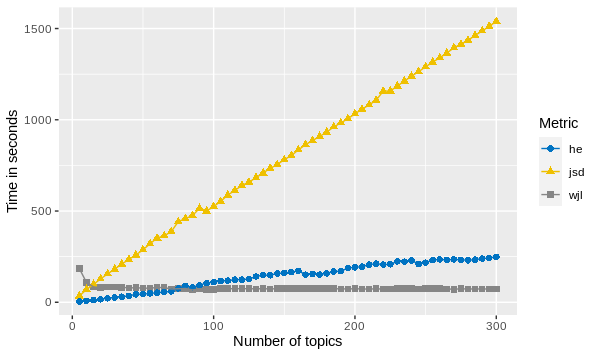
\includegraphics[width=0.8\linewidth]{time_comp.png}
    \caption{Time needed (in milliseconds) to perform the document similarity \\ task using similarity metrics in a corpus of $10^4$ synthetic documents }
    \label{fig:compare_time_metric}
\end{figure}

These results reinforce us in the use of probabilistic topic models to facilitate the exploration of large collections of multilingual documents. The knowledge inferred by these models to automatically group semantically related documents is highly sensitive to the texts used in their training. Their ability to generalize such knowledge only seems to make sense in one direction: with texts whose length is equal to or longer than those used during training. This allows us to conclude that, for example, the knowledge extracted from the topics inferred from a collection of tweets (texts of no more than 260 characters), cannot be extended to automatically classify, for example, blog posts (more than 300 characters). If we assume that the complexity of a text increases as its length increases, the logic used to infer topics is unable to capture more complex knowledge than was proposed during training.


\section{Summary}
\label{sec:crosslingual-summary}

In this chapter we have described documents based on topic models that create a unique space of representation between different languages. Topics are created independently for each language, and are projected on concepts instead of words. On concept-based representations, documents in different languages coexist together and can be related. This addresses the last research objective of this thesis (R06, \textit{define a transformation of the topic-based annotations to create a unique representational space out of the particularities from each language}). Representations are analyzed in classification and information retrieval tasks on multilingual document collections. As expected, the performance in terms of accuracy is not as good as that of the approach based on prior knowledge (i.e. topics previously aligned by documents annotated with categories). However, in terms of coverage, the performance of the unsupervised approach is much greater than that offered by the semi-supervised approach, to the point of offering better overall performance (i.e f1) in classification tasks. 
In addition, the algorithm has proved to perform close to the semi-supervised algorithm in the information retrieval task, which makes us think that the process of topic annotation by set of synonyms should be improved to filter those elements that are not sufficiently representative. For example by defining a mechanism similar to the one used to create "stopwords" to identify \textit{"stopconcepts"}. 

In order to perform the evaluations, the new representation system was implemented in our libAIry framework. This extension, together with those described in chapters \ref{ch:explainability} and \ref{ch:comparisons}, cover the last technical objective of this thesis (T04, \textit{create a system capable of finding similar documents automatically}). 